%======================================================================
\chapter{Control Algorithms}
\label{ch: Chapter3}
%======================================================================
This chapter discusses the three control algorithms used in the experiment.  These are linear quadric regulator (LQR) 
%----------------------------------------------------------------------
\section{LQR}
%----------------------------------------------------------------------

    After creating the system model
    \begin{align*}
        \dot{\mathbf{x}} = \mathbf{A}\mathbf{x} + \mathbf{B}\mathbf{u}
    \end{align*}
    use the state feedback law
    \begin{center}
        $\mathbf{u} = -\mathbf{K}\mathbf{x}$
    \end{center}
    to minimize the quadratic cost function:
    \begin{align*}
        J(\mathbf{u}) = \int_0^\infty (\mathbf{x}^T\mathbf{Q}\mathbf{x} + \mathbf{u}^T\mathbf{R}\mathbf{u} + 2\mathbf{x}^T\mathbf{N}\mathbf{u})\mathrm{dt}
    \end{align*}
    Find the solution $\mathbf{S}$ to the Riccati equation
    \begin{align*}
        \mathbf{A}^T\mathbf{S}+\mathbf{SA}-(\mathbf{SB}+\mathbf{N})\mathbf{R}^{-1}(\mathbf{B}^T\mathbf{S}+\mathbf{N}^T)+\mathbf{Q}=0
    \end{align*}    
    Calculate gain, $\mathbf{K}$
    \begin{center}
        $\mathbf{K}=\mathbf{R}^{-1}(\mathbf{B}^T\mathbf{S}+\mathbf{N}^T)$
    \end{center}

%----------------------------------------------------------------------
\section{LQG}
%----------------------------------------------------------------------

\begin{itemize}   
    \item Utilizes gain calculated in LQR
    \item Added Kalman filter to reduce external disturbances to the system
\end{itemize}
%----------------------------------------------------------------------
\section{ADP}
%----------------------------------------------------------------------

\begin{figure}[!htbp]
    \centering
    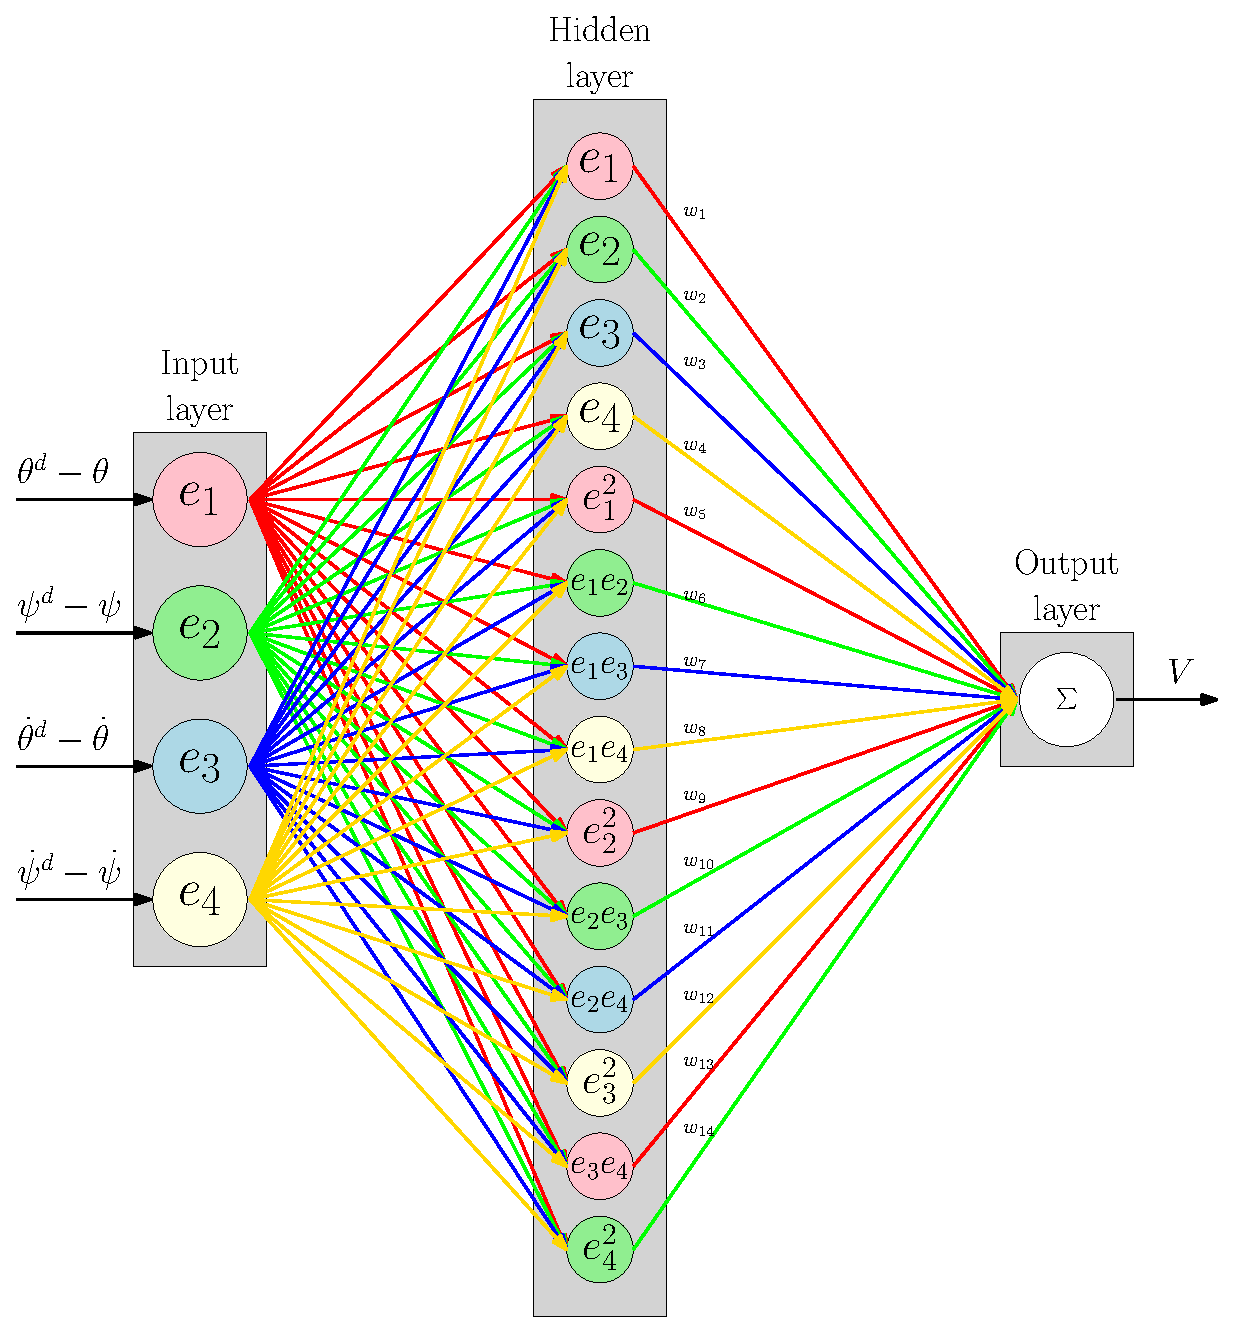
\includegraphics[width=.46\textwidth,keepaspectratio=true]{figs/ipe/ADP_Neural_Network.eps}
    \label{fig:ADP_Neural_Network}
    \caption{Input nodes are connected to the hidden layer and then to the output layer.}
\end{figure}
\begin{figure}[!htbp]
    \centering
    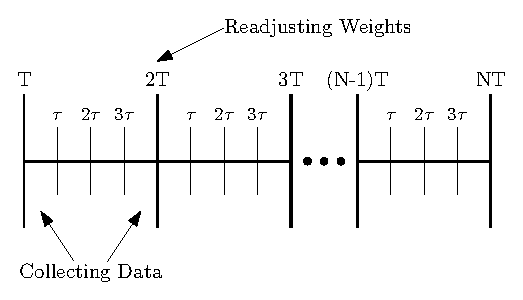
\includegraphics[width=.46\textwidth,keepaspectratio=true]{figs/ipe/ADP_Samples.eps}
    \label{fig:ADP_Samples}
    \caption{Data is collected for every $\tau$ seconds and then the weights are adjusted every $T$ seconds.}
\end{figure}

%----------------------------------------------------------------------
\section{Improvements}
Most of these algorithms are typically implemented only using proportional gain which causes steady-state error to certain input signals in some systems.  In our case, we experience steady-state error for a step input.  To reduce this, the type of the controller needs to be increased by adding an integrator.  We solve this problem by implementing a PI controller where LQR and ADP are used to find the optimal proportional and integral gain.\\
This is done by creating an augmented matrix with A and B with different dimensions

%----------------------------------------------------------------------



%%% Local Variables:
%%% mode: latex
%%% TeX-master: "../finalReport"
%%% End:
